\documentclass[12pt]{article}
\usepackage[english]{babel}
\usepackage[utf8]{inputenc}

%% Pointer to 'default' preamble
% pacakages and definitions

\usepackage{geometry}
\geometry{
	letterpaper, 
	portrait, 
	top=.75in,
	left=.8in,
	right=.75in,
	bottom=.5in		} 	% Page Margins
	
%% additional packages for nice things
\usepackage{amsmath} 	% for most math
\usepackage{commath} 	% for abs
\usepackage{lastpage}	% for page count
\usepackage{amssymb} 	% for therefore
\usepackage{graphicx} 	% for image handling
\usepackage{wrapfig} 	% wrap figures
\usepackage[none]{hyphenat} % for no hyphenations
\usepackage{array} 		% for >{} column characterisctis
\usepackage{physics} 	% for easier derivative \dv....
\usepackage{tikz} 		% for graphic@!
\usepackage{circuitikz} % for circuits!
\usetikzlibrary{arrows.meta} % for loads
\usepackage[thicklines]{cancel}	% for cancels
\usepackage{xcolor}		% for color cancels
\usepackage[per-mode=fraction]{siunitx} % for si units and num
\sisetup{group-separator = {,}, group-minimum-digits = 3} % additional si unit table functionality

\usepackage{fancyhdr} 	% for header
\usepackage{comment}	% for ability to comment out large sections
\usepackage{multicol}	% for multiple columns using multicols
\usepackage[framed,numbered]{matlab-prettifier} % matlab sytle listing
\usepackage{marvosym} 	% for boltsymbol lightning
\usepackage{pdflscape} 	% for various landscape pages in portrait docs.
%\usepackage{float}
\usepackage{fancyvrb}	% for Verbatim (a tab respecting verbatim)
\usepackage{enumitem}	% for [resume] functionality of enumerate
\usepackage{spreadtab} 	% for using formulas in tables}
\usepackage{numprint}	% for number format in spread tab
\usepackage{subcaption} % for subfigures with captions
\usepackage[normalem]{ulem} % for strike through sout

% for row colors in tables....
\usepackage{color, colortbl}
\definecolor{G1}{gray}{0.9}
\definecolor{G2}{rgb}{1,0.88,1}%{gray}{0.6}
\definecolor{G3}{rgb}{0.88,1,1}

% For table formatting
\usepackage{booktabs}
\renewcommand{\arraystretch}{1.2}
\usepackage{floatrow}
\floatsetup[table]{capposition=top} % put table captions on top of tables

% Caption formating footnotesize ~ 10 pt in a 12 pt document
\usepackage[font={small}]{caption}

%% package config 
\sisetup{output-exponent-marker=\ensuremath{\mathrm{E}}} % for engineer E
\renewcommand{\CancelColor}{\color{red}}	% for color cancels
\lstset{aboveskip=2pt,belowskip=2pt} % for more compact table
%\arraycolsep=1.4pt\def
\setlength{\parindent}{0cm} % Remove indentation from paragraphs
\setlength{\columnsep}{0.5cm}
\lstset{
	style      = Matlab-editor,
	basicstyle = \ttfamily\footnotesize, % if you want to use Courier - not really used?
}
\renewcommand*{\pd}[3][]{\ensuremath{\dfrac{\partial^{#1} #2}{\partial #3}}} % for larger pd fracs
\renewcommand{\real}[1]{\mathbb{R}\left\{ #1 \right\}}	% for REAL symbol
\newcommand{\imag}[1]{\mathbb{I}\left\{ #1 \right\}}	% for IMAG symbol
\definecolor{m}{rgb}{1,0,1}	% for MATLAB matching magenta
	
%% custom macros
\newcommand\numberthis{\addtocounter{equation}{1}\tag{\theequation}} % for simple \numberthis command

\newcommand{\equal}{=} % so circuitikz can have an = in the labels
\newcolumntype{L}[1]{>{\raggedright\let\newline\\\arraybackslash\hspace{0pt}}m{#1}}
\newcolumntype{C}[1]{>{\centering\let\newline\\\arraybackslash\hspace{0pt}}m{#1}}
\newcolumntype{R}[1]{>{\raggedleft\let\newline\\\arraybackslash\hspace{0pt}}m{#1}}

%% Header
\pagestyle{fancy} % for header stuffs
\fancyhf{}
% spacing
\headheight 29 pt
\headsep 6 pt

%% Header
\rhead{Thad Haines \\ Page \thepage\ of \pageref{LastPage}}
\chead{PST and VTS \\ - DRAFT 4 -}
\lhead{Research \\ 08/04/20}
\usepackage{minted}
\usepackage{setspace}
\begin{document}
\onehalfspacing
\paragraph{Purpose} \ \\
This document is meant to explain PST additions and alterations created to accommodate VTS (variable time stepping).
While the current method works, it may change in the future.

\paragraph{Solver Control Array} \ \\
Theoretically, a user will only have to add a \verb|solver_con| to a valid data file to use variable time step methods.
If a \verb|solver_con| is not specified, Huen's method is used for all time blocks (i.e. default PST behavior).

Between each \verb|sw_con| entry, a \emph{time block} is created that is then solved using a the defined solution method in the \verb|solver_con|.
As such, the \verb|solver_con| array has 1 less row than the \verb|sw_con| array.
An example \verb|solver_con| array (with code comments) is shown below.
\begin{minted}[
		frame=lines,
		framesep=2mm,
		baselinestretch=1.2,
		bgcolor=gray!13,
		fontsize=\footnotesize,
		%linenos,
		breaklines
		]{MATLAB}
%% solver_con format
% A cell with a solver method in each row corresponding to the specified
% 'time blocks' defined in sw_con
%
% Valid solver names:
% huens - Fixed time step default to PST
% ode113 - works well during transients, consistent # of slns, time step stays relatively small
% ode15s - large number of slns during init, time step increases to reasonable size
% ode23 - realtively consistent # of required slns, timstep doesn't get very large
% ode23s - many iterations per step - not efficient...
% ode23t - occasionally hundereds of iterations, sometimes not... decent
% ode23tb - similar to 23t, sometimes more large solution counts

solver_con ={ ...
    'huens'; % pre fault - fault
    'huens'; % fault - post fault 1
    'huens'; % post fault 1 - post fault 2
    'huens'; % post fault 2 - sw_con row 5
    'huens'; % sw_con row 5 - sw_con row 6 
    'ode23t'; % sw_con row 6  - sw_con row 7  (end)
    };
\end{minted}

As of this writing, the pstSETO version uses the \verb|s_simu_BatchVTS| script to perform variable time stepping methods.
This script will likely replace the \verb|s_simu| script in the main PST4 folder after versioning is complete.\\


\pagebreak
\paragraph{MATLAB ODE solver} \ \\
The variable time step implementation in PST revolves around using the built in MATLAB ODE solvers.
All these methods perform actions depicted in the following block diagram.

\begin{center}
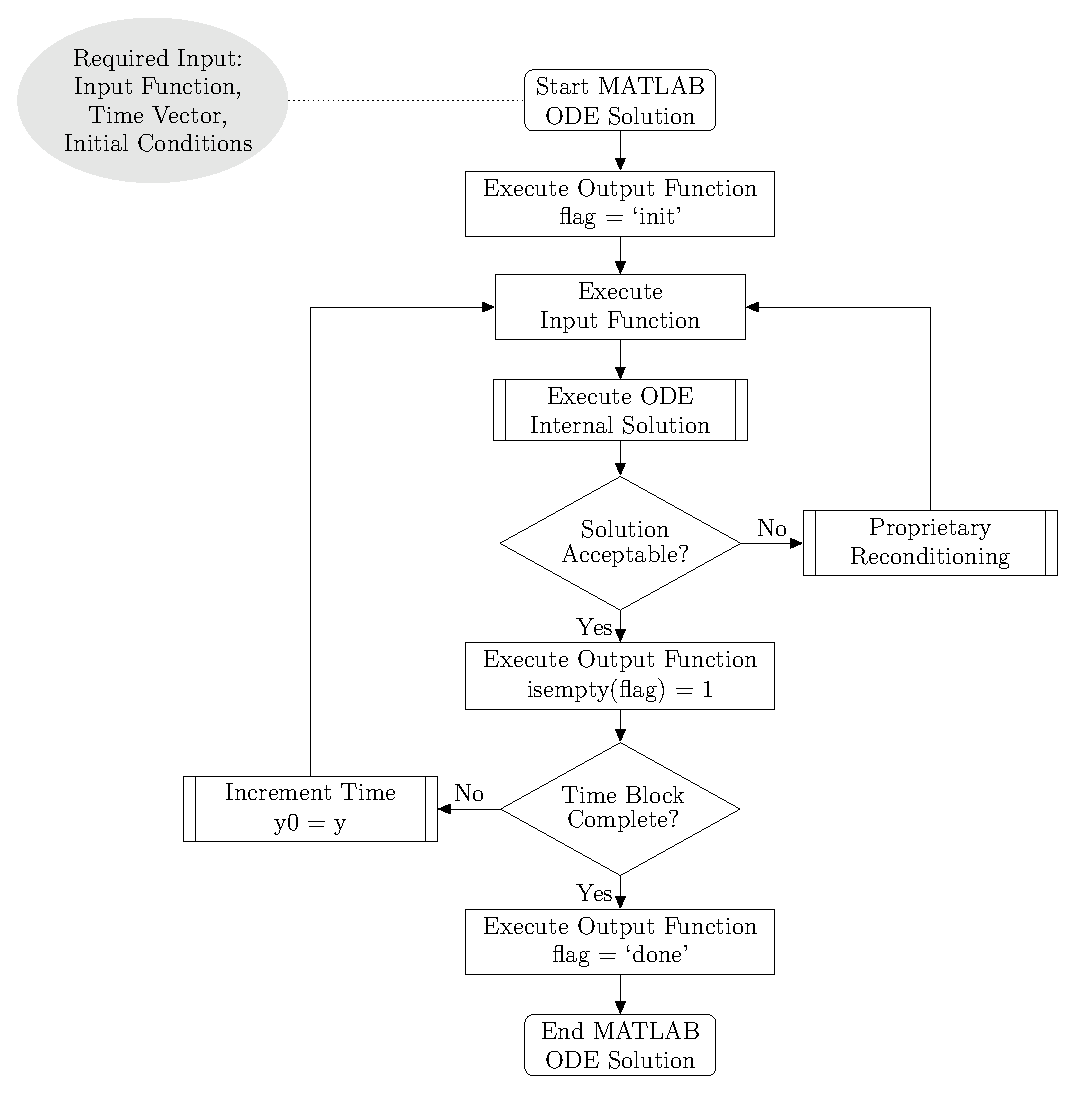
\includegraphics[width=.8\linewidth]{./../200804-ODEblockDiagram/200804-ODEblockDiagram}
\end{center}

The input to an ODE solver include, an input function, a time interval (time block), initial conditions, and solver options.
The current options used for VTS are shown below and deal with error tolerance levels, initial step size, max step size, and an Output function.

\begin{minted}[
		frame=lines,
		framesep=2mm,
		baselinestretch=1.2,
		bgcolor=gray!13,
		fontsize=\footnotesize,
	%	linenos,
		breaklines
				]{MATLAB}
% Configure ODE settings
%options = odeset('RelTol',1e-3,'AbsTol',1e-6); % MATLAB default settings
options = odeset('RelTol',1e-4,'AbsTol',1e-7, ...
    'InitialStep', 1/60/4, ...
    'MaxStep',60, ...
    'OutputFcn',outputFcn); % set 'OutputFcn' to function handle
\end{minted}

\pagebreak
\paragraph{vtsInputFcn} \ \\
The slightly abbreviated (mostly complete) input function is shown below.
\begin{minted}[
		frame=lines,
		framesep=2mm,
		baselinestretch=1.2,
		bgcolor=gray!13,
		fontsize=\footnotesize,
	%	linenos,
		breaklines
				]{MATLAB}
function [dxVec] = vtsInputFcn(t, y)
% VTSINPUTFCN passed to ODE solver to perfrom required step operations
%
%   NOTES: Updates and returns g.vts.dxVec
%
%   Input:
%   t - simulation time
%   y - solution vector (initial conditions)
%
%   Output:
%   dxVec - requried derivative vector for ODE solver
global g

%% call handleStDx with flag==2 to update global states with newest passed in soln.
% write slnVec vector of values to associated states at index k
% i.e. update states at g.vts.dataN with newest solution
handleStDx(g.vts.dataN, y, 2)

%% Start initStep action ==================================================
initStep(g.vts.dataN)

%% Start of Network Solution ==============================================
networkSolutionVTS(g.vts.dataN, t)

%% Start Dynamic Solution =================================================
dynamicSolution(g.vts.dataN )

%% Start of DC solution ===================================================
dcSolution(g.vts.dataN )

%% save first network solution
if g.vts.iter == 0
    handleNetworkSln(g.vts.dataN ,1)
end

g.vts.iter = g.vts.iter + 1; % increment solution iteration number

handleStDx(g.vts.dataN , [], 1) % update g.vts.dxVec
dxVec = g.vts.dxVec; % return updated derivative vector
end % end vtsInputFcn
\end{minted}

\pagebreak

\paragraph{vtsOutputFcn} \ \\
The slightly abbreviated output function is shown below.
\begin{minted}[
		frame=lines,
		framesep=2mm,
		baselinestretch=1.2,
		bgcolor=gray!13,
		fontsize=\footnotesize,
	%	linenos,
		breaklines
				]{MATLAB}
function status = vtsOutputFcn(t,y,flag)
% VTSOUTPUTFCN performs associated flag actions with ODE solvers.
%
%   Input:
%   t - simulation time
%   y - solution vector
%   flag - dictate function action
%
%   Output:
%   status - required for normal operation (return 1 to stop)

global g 
status = 0; % required for normal operation

if isempty(flag) % normal step completion
    % restore network to initial solution
    handleNetworkSln(g.vts.dataN ,2) % may cause issues with DC.
    
    monitorSolution(g.vts.dataN); % Perform Line Monitoring and Area Calculations 
    
    %% Live plot call
    if g.sys.livePlotFlag
        livePlot(g.vts.dataN)
    end
    
    % after each successful integration step by ODE solver:
    g.vts.dataN = g.vts.dataN+1;    % increment logged data index 'dataN'
    g.sys.t(g.vts.dataN) = t;       % log step time
    g.vts.stVec = y;                % update state vector
    handleStDx(g.vts.dataN, y, 2)   % place new solution results into associated globals
    
    g.vts.tot_iter = g.vts.tot_iter + g.vts.iter;   % update total iterations
    g.vts.slns(g.vts.dataN) = g.vts.iter;           % log solution step iterations
    g.vts.iter = 0;                                 % reset iteration counter
    
elseif flag(1) == 'i' 
    % init solver for new time block
    g.sys.t(g.vts.dataN) = t(1);    % log step time
    handleStDx(g.vts.dataN, y, 2)   % set initial conditions
  
elseif flag(1) == 'd'
    % only debug screen output at the moment
end % end if
end % end function
\end{minted}

\pagebreak
\paragraph{Simulation Loop}
The complete simulation loop code is shown below.
This code was copied from \verb|s_simu_BatchVTS| with corresponding line numbers.

\begin{minted}[
		frame=lines,
		framesep=2mm,
		baselinestretch=1.2,
		bgcolor=gray!13,
		fontsize=\footnotesize,
		linenos,
		firstnumber=362,
		breaklines
				]{MATLAB}
%% Simulation loop start
warning('*** Simulation Loop Start')
for simTblock = 1:size(g.vts.t_block)
    
    g.vts.t_blockN = simTblock;
    g.k.ks = simTblock; % required for huen's solution method.
    
    if ~isempty(g.vts.solver_con)
        odeName = g.vts.solver_con{g.vts.t_blockN};
    else
        odeName = 'huens'; % default PST solver
    end
    
    if strcmp( odeName, 'huens')
        % use standard PST huens method
        fprintf('*** Using Huen''s integration method for time block %d\n*** t=[%7.4f, %7.4f]\n', ...
            simTblock, g.vts.fts{simTblock}(1), g.vts.fts{simTblock}(end))
        
        % add fixed time vector to system time vector
        nSteps = length(g.vts.fts{simTblock});
        g.sys.t(g.vts.dataN:g.vts.dataN+nSteps-1) = g.vts.fts{simTblock};
        
        % account for pretictor last step time check
        g.sys.t(g.vts.dataN+nSteps) = g.sys.t(g.vts.dataN+nSteps-1)+ g.sys.sw_con(simTblock,7);
        
        for cur_Step = 1:nSteps
            k = g.vts.dataN;
            j = k+1;
            
            % display k and t at every first, last, and 50th step
            if ( mod(k,50)==0 ) || cur_Step == 1 || cur_Step == nSteps
                fprintf('*** k = %5d, \tt(k) = %7.4f\n',k,g.sys.t(k)) % DEBUG
            end
            
            %% Time step start
            initStep(k)
            
            %% Predictor Solution =========================================
            networkSolutionVTS(k, g.sys.t(k))
            monitorSolution(k);
            dynamicSolution(k)
            dcSolution(k)
            predictorIntegration(k, j, g.k.h_sol)   % g.k.h_sol updated i_simu
            
            %% Corrector Solution =========================================
            networkSolutionVTS(j, g.sys.t(j))
            dynamicSolution(j)
            dcSolution(j)
            correctorIntegration(k, j, g.k.h_sol)
            
            % most recent network solution based on completely calculated states is k
            monitorSolution(k);
            %% Live plot call
            if g.sys.livePlotFlag
                livePlot(k)
            end
            
            g.vts.dataN = j;                        % increment data counter
            g.vts.tot_iter = g.vts.tot_iter  + 2;   % increment total solution counter
            g.vts.slns(g.vts.dataN) = 2;            % track step solution
        end
        % Account for next time block using VTS
        handleStDx(j, [], 3) % update g.vts.stVec to initial conditions of states
        handleStDx(k, [], 1) % update g.vts.dxVec to initial conditions of derivatives 
        
    else % use given variable method
        fprintf('*** Using %s integration method for time block %d\n*** t=[%7.4f, %7.4f]\n', ...
            odeName, simTblock, g.vts.t_block(simTblock, 1), g.vts.t_block(simTblock, 2))
        
        % feval used for ODE call - could be replaced with if statements.
        feval(odeName, inputFcn, g.vts.t_block(simTblock,:), g.vts.stVec , options);
        
        % Alternative example of using actual function name:
        %ode113(inputFcn, g.vts.t_block(simTblock,:), g.vts.stVec , options);
    end
    
end% end simulation loop
\end{minted}

\pagebreak
\paragraph{Functions for Variable Time Step Integration} \ \\
A number of new functions were created to allow for VTS to be integrated into PST and collected in the \verb|test| folder of the main SETO version directory.
Some functions were simply portions of code previously located in \verb|s_simu| and placed into a function for ease of use and clarity of code flow, while others were created to handle data or perform other tasks specifically related to VTS.
The following sub paragraphs provide some information about such functions that have not been previously introduced.

%+=================================================+++++++++++++++++++++++++++++++++++++++++++++++++++++++++++++++++++++++++++++++++++++++++++++++++++++++++++++++++++++++++++++++++++++++++++++++++++++++=================================================================


%==========================================================
\subparagraph{s\_simu\_BatchTestF} \ \\
The \verb|s_simu_BatchTestF| script is a modified version of \verb|s_simu_Batch| that was used to test the new functions used in non-linear simulation outside of the variable time step process.
As the VTS method appears to work, this script will most likely go away as it has served its purpose.

%==========================================================
\subparagraph{s\_simu\_BatchVTS} \ \\
The \verb|s_simu_BatchVTS| script is a functionalized \verb|s_simu_Batch| with elements from \verb|s_simu| that prompt user input re-introduced.
To enter \emph{stand alone mode} (where the user is prompted for input), simply run this script after issuing the \verb|clear all; close all| commands.
While being able to operate in stand alone mode, it is also able to run in \emph{batch mode} where it assumes the data file to run is the \verb|DataFile.m| in the root PST directory.
This script performs optional VTS simulation and is slated to replace \verb|s_simu| once PST SETO becomes PST 4.0.


%==========================================================
\subparagraph{initZeros} \ \\
A large amount of code ($\approx$400 lines) in \verb|s_simu| was dedicated to initializing zeros for data to be written to during non-linear simulation.
This code has been collected into the \verb|initZeros| function with inputs defining the desired length of vectors for normally logged data and DC data.

\begin{minted}[
		frame=lines,
		framesep=2mm,
		baselinestretch=1.2,
		bgcolor=gray!13,
		fontsize=\footnotesize,
	%	linenos,
		breaklines
				]{MATLAB}
function initZeros(k, kdc)
% INITZEROS Creates zero arrays for logged values based on passed in input
%
%   Input:
%   k - total number of time steps in the simulation
%   kdc - total number of DC time steps in the simulation
\end{minted}

%==========================================================
\subparagraph{initNLsim} \ \\
The \verb|initNLsim| function is a collection of code from \verb|s_simu| that performs initialization operations before a non-linear simulation.
This is essentially the creation of the various Y-matrices used for fault conditions and the calling of the dynamic models with the input flag set to 0.

\pagebreak
%==========================================================
\subparagraph{initTblocks} \ \\
The \verb|initiTblocks| function analyzes the global \verb|sw_con| and \verb|solver_con| to create appropriate \emph{time blocks} that are used in VTS simulation.
Any fixed time vectors associated with time blocks that use Huen's method are also created.
Care was taken to ensure a unique time vector (no duplicate time points).
With the option to switch between fixed step and variable step  methods, this method may require slight modifications/refinements.

%==========================================================
\subparagraph{initStep} \ \\
Code from \verb|s_simu| that was performed at the begining of each solution step was collected into \verb|initStep|.
Operations are related to setting values for the next step equal to current values for mechanical powers and DC currents, as well as handling machine trip flags.


%==========================================================
\subparagraph{networkSolution} \ \\
The \verb|networkSolution| function is a collection of code from \verb|s_simu| dealing with calls to dynamic models with the flag set to 1 and Y-matrix switching.
The call to \verb|i_simu| (which updates \verb|g.k.h_sol|) is located in this function.
The input to this function is the data index on which to operate.

%==========================================================
\paragraph{networkSolutionVTS} \ \\
The \verb|networkSolutionVTS| function is essentially the same as the \verb|networkSolution| function, except instead of relying on index number to switch Y-matricies, the switching is done based on passed in simulation time.
This was a required change when using VTS as the previous method relied on a known number of steps between switching events, and that is no longer a reality.


%==========================================================
\subparagraph{dynamicSolution} \ \\
As the name implies, the \verb|dynamicSolution| function performs the dynamic model calculations at data index \verb|k| by calling each required model with the input flag set to 2.
This functionalized code is again taken directly from \verb|s_simu|.


%==========================================================
\subparagraph{dcSolution} \ \\
The portion of \verb|s_simu| that integrates DC values at 10 times the rate of the normal time step was moved into the \verb|dcSolution| function.
This has not been tested with VTS, but was functionalized to enable future developement.
It \emph{should} work as normal when using Huen's method, but is untested as of this writing.

\pagebreak
%==========================================================
\subparagraph{monitorSolution} \ \\
The \verb|monitorSolution| function takes a single input that defines the data index used to calculate any user defined line monitoring values, average system/area frequencies, and values for any defined areas.
It should be noted that these calculations are mostly based on complex voltages that are calculated during the network solution.

%==========================================================
\subparagraph{predictorIntegration} \ \\
The \verb|predictorIntegration| function performs the predictor (forward Euler) integration step of the simulation loop.
The code was taken directly from \verb|s_simu| and uses the same variable names.

\begin{minted}[
		frame=lines,
		framesep=2mm,
		baselinestretch=1.2,
		bgcolor=gray!13,
		fontsize=\footnotesize,
	%	linenos,
		breaklines
				]{MATLAB}
function predictorIntegration(k, j, h_sol)
% PREDICTORINTEGRATION Performs  x(j) = x(k) + h_sol*dx(k)
%
%   Input:
%   k - data index for 'n'
%   j - data index for 'n+1'
%   h_sol - time between k and j
\end{minted}


%==========================================================
\subparagraph{correctorIntegration} \ \\
As shown in the code except below, the \verb|correctorIntegration| function performs the corrector integration step of the simulation loop to calculate the next accepted value of integrated states.
The executed code was taken directly from \verb|s_simu|.

\begin{minted}[
		frame=lines,
		framesep=2mm,
		baselinestretch=1.2,
		bgcolor=gray!13,
		fontsize=\footnotesize,
	%	linenos,
		breaklines
				]{MATLAB}
function correctorIntegration(k, j, h_sol)
% CORRECTORINTEGRATION Performs x(j) = x(k) + h_sol*(dx(j) + dx(k))/2
%
%   Input:
%   k - data index for 'n'
%   j - data index for 'n+1'
%   h_sol - time between k and j
\end{minted}

It should be noted that the two `Integration' functions write new states to the same \verb|j| data index.
Additionally, the \verb|h_sol| value is updated in \verb|i_simu| (called during the network solution) from the index of \verb|ks| referencing an \verb|h| array containing time step lengths$\ldots$\ 
While this process seemed unnecessarily confusing and sort of  round-about, it has not been changed as of this writing.

\pagebreak
%==========================================================
\subparagraph{handleStDx} \ \\
The \verb|handleStDx| function was created to perform the required state and derivative handling to enable the use internal MATLAB ODE solvers.
Its general operation is probably best described via the internal function documentation provided below.

\begin{minted}[
		frame=lines,
		framesep=2mm,
		baselinestretch=1.2,
		bgcolor=gray!13,
		fontsize=\footnotesize,
	%	linenos,
		breaklines
				]{MATLAB}
function handleStDx(k, slnVec, flag)
% HANDLESTDX Performs required state and derivative handling for ODE solvers
%
%   NOTES:  Requires state and derivative values are in the same g.(x) field.
%           Not all flags require same input.
%
%   Input:
%   k - data index
%   flag - choose between operations
%           0 - initialize state and derivative cell array, count states
%           1 - update g.vts.dxVec with col k of derivative fields
%           2 - write slnVec vector of values to associated states at index k
%           3 - update g.vts.stVec with col k of state fields
%   snlVec - Input used to populate states with new values
\end{minted}

The new global structure created in the SETO version of PST enables this function to complete the stated operations by relying heavily on dynamic field names. 
Essentially, all required field names, sub-field names, and states are collected into a cell (flag operation 0) that is then iterated through to collect data from, or write data to the appropriate location (all other flag operations).\\

The usefulness of \verb|handleStDx| is that the standard MATLAB ODE solvers require a single derivative vector as a returned value from some passed in `input function', and each PST model calculates derivatives and places them into various globals. 
Thus, a derivative collection algorithm was needed (flag operation 1).
Once the ODE solver finishes a step, the returned solution vector (of integrated states) must then be parsed into the global state variables associated with the supplied derivatives (flag operation 2).
At the beginning of time blocks that use the MATLAB ODE solvers, an initial conditions vector of all the states related to the derivative vector is required (flag operation 3).\\

To avoid handling function output, global vectors \verb|g.vts.dxVec| and \verb|g.vts.stVec| are used to hold updated derivative and state vector information.

It should be noted that original PST globals follow the same data structure,
however, new models (such as AGC and pwrmod/ivmmmod) use a slightly different data structure and must be handled in a slightly different way.
As of this writing AGC and pwrmod functionality has been added to \verb|handleStDx| and it seems very possible to add more models that require integration as they arise.

\pagebreak
%==========================================================
\subparagraph{handleNetworkSln} \ \\
The \verb|handleNetworkSln| function was created to store, and restore, calculated values set to globals during a network solution.
The purpose of this function was to allow for the first network solution performed each step to be carried forward after multiple other network solutions may over-write the calculated values at the same data index.
This over-writing may occur during the MATLAB ODE solvers repeated call to the input function.
As shown below, \verb|handlNetworkSln| takes a data index \verb|k| and an operation \verb|flag| as inputs.
\begin{minted}[
		frame=lines,
		framesep=2mm,
		baselinestretch=1.2,
		bgcolor=gray!13,
		fontsize=\footnotesize,
	%	linenos,
		breaklines
				]{MATLAB}
function handleNetworkSln(k, flag)
% HANDLENETWORKSLN saves or restores the network solution at data index k
%
%   NOTES: Used to reset the newtork values to the initial solution in VTS.
%
%   Input:
%   k - data index to log from and restore to
%   flag - choose funtion operation
%       0 - initialize globals used to store data
%       1 - collect newtork solution values from index k into a global vector
%       2 - write stored network solution vector to network globals data at index k
\end{minted}

%==========================================================
\subparagraph{trimLogs} \ \\
As there is no way to accurately predict the amount of (length of) data to be logged during a variable time step simulation, more space is allocated (20x the amount from a fixed step simulation) and then all logged values are trimmed to the proper length post simulation.
It should be noted that this 20x size allocation was arbitrary and will probably be altered in the future as actual extended term simulation using VTS typically requires fewer steps than a fixed step method.
However, if not enough space is allocated the simulation will crash.

\begin{minted}[
		frame=lines,
		framesep=2mm,
		baselinestretch=1.2,
		bgcolor=gray!13,
		fontsize=\footnotesize,
	%	linenos,
		breaklines
				]{MATLAB}
function trimLogs(k)
% TRIMLOGS trims logged data to input index k.
%
%   NOTES: nCell not made via logicals - may lead to errors if fields not initialized (i.e. model not used). Issue not encountered yet, but seems possible
%
%   Input:
%   k - data index
\end{minted} 

%==========================================================
\subparagraph{standAlonePlot} \ \\
The \verb|standAlonePlot| function is the updated plotting routine based on user input previously found at the end \verb|s_simu|.
After a completed simulation, it is called from \verb|s_simu_BatchVTS| if stand alone mode is detected.


%==========================================================
%\subparagraph{vtsInputFcn and vtsOutputFcn} \ \\
%These functions were described earlier.


\begin{comment}
Document Section 'templates'
%==========================================================
\subparagraph{FcnName} \ \\
FcnDescription
\begin{minted}[
		frame=lines,
		framesep=2mm,
		baselinestretch=1.2,
		bgcolor=gray!13,
		fontsize=\footnotesize,
	%	linenos,
		breaklines
				]{MATLAB}
PasteNewCodeHere
\end{minted}

%==========================================================
\begin{minted}[
		frame=lines,
		framesep=2mm,
		baselinestretch=1.2,
		bgcolor=gray!13,
		fontsize=\footnotesize,
	%	linenos,
		breaklines
				]{MATLAB}
PasteNewCodeHere
\end{minted}
%==========================================================

\end{comment}


\end{document}
